\documentclass{article}
\usepackage{CJKutf8}
\usepackage{multirow}
\usepackage[cmex10]{amsmath}
\usepackage{listings}
\usepackage{algorithmic}
\usepackage{algorithm}
\usepackage{epsfig}
\usepackage{amsopn}
\usepackage{subfigure}
\usepackage{cite}
\usepackage{courier}
\makeatletter
\makeatother
\begin{CJK}{UTF8}{gbsn}
\usepackage[framed,autolinebreaks,useliterate]{mcode}

\usepackage{graphicx}
\begin{document}
\title{通信与网络第四次仿真练习作业\\匹配滤波与最佳接收 }
\author{王亭午,2012011018,无210班}
\date{2015年11月14号}
\maketitle
\section{问题一}
编写一个含QAM传输的发送和接收模块。分别采用复基带仿真和实带通仿真两种形式:复基带仿真时过采样率为4倍,实带通仿真时过采样率为20倍, 实带通仿真时, 载波频率为符号率的4倍,发端采用滚降系数0.5的根号升余弦滤波器。画出Eb/N0=15dB时的接收波形(收滤波前),取100个采样。画出发端输出的眼图和收端过匹配滤波后的眼图(画眼图时不加噪声),统计误符号率和误比特率与Eb/N0的关系,画出曲线, 与理论计算的曲线相对比。\\
\textbf{答案}:我仿真的是最为普遍的16QAM传输。之所以选择16QAM是因为我在另外一门课,通信系统课中,曾经仿真过4QAM,因此这里尝试仿真一个更加复杂一点的。
\subsection{实通带传输}
\textbf{答案}:实通带传输的结果为图1-图5,在实验中我们采用了2500个符号,每秒钟送出一个符号。核心代码如下:
\begin{lstlisting}
% the signal then pass a sqrt raise cosine singal filter. The over sample 
% rate is 20, and the alpha is 0.5. Thus the original 250 points is no 
% sampled into 250 * 20 = 50 data
I_s = rcosflt(I, 1, 20, 'sqrt', 0.5); I_s = I_s(61 : end - 60);
Q_s = rcosflt(Q, 1, 20, 'sqrt', 0.5); Q_s = Q_s(61 : end - 60);

w = 2 * pi * 4;  % one sample sent in 1s, therefore 4 is the freq
QAM_Signal = I_s' .* cos(w * t) - Q_s' .* sin(w * t);  % it is the signal
\end{lstlisting}
在上面的代码中,我们使用升余弦滤波器进行成型,然后加载在了我们指定的通带载波上。输出的眼图在图2中。\\
接下来我们进行解调,解调的代码如下,这是一个相干解调:
\begin{lstlisting}
% Calculate the recover result when no noise is around
I_received_noNoise = 2 * (QAM_Signal) .* cos(w*t);
Q_received_noNoise = 2 * (QAM_Signal) .* (-sin(w*t));

I_received_noNoise = rcosflt(I_received_noNoise, 1, 20, 'sqrt/Fs', 0.5);
I_received_noNoise = I_received_noNoise(61: end - 61);
Q_received_noNoise = rcosflt(Q_received_noNoise, 1, 20, 'sqrt/Fs', 0.5);
Q_received_noNoise = Q_received_noNoise(61: end - 61);
\end{lstlisting}
通过和自己的载波相乘,我们恢复出最初发射的信号,可以看到,在图2中,信号已经是非常整齐的了。\\
随后是我们的误码率判断,代码如下。
\begin{lstlisting}
% calculate the bit error
pb = zeros(16, 1);
pb_theory = zeros(16, 1);
for k = 1:16
    pb(k) = 1 - sum(Output(k,:) == x) / N;
end
figure; subplot(2,1,1); grid on;
plot(pb); title('The simulated BER curve'); grid on;
for k = 1:16
    pb_theory(k) = 4 / 4 * (1 - 1 / 4) * qfunc(sqrt(3*4/15*10^(k / 10)));
    %pb_theory(k) = 2*(4-1)/4*qfunc(sqrt(6*2/15*k));
end
subplot(2,1,2); plot(pb_theory); grid on;
title('The theoretical BER curve');

% calculate the symbol error
k_bits = 4;  % 4 bits
ps = zeros(16, 1);
ps_theory = zeros(16, 1);
for k = 1:16
    error = 0;
    for i = 1: 1: numSample
        if all(Output(k, 1 + (i - 1) * 4 : i * 4) == x(1 + (i - 1) * 4 : i * 4))
            continue
        else
            error = error + 1;
        end
    end
    ps(k) = error / numSample;
end
figure; subplot(2,1,1); grid on;
plot(ps); title('The simulated SER curve'); grid on;
for k = 1:16
    ps_theory(k) = 1 - (1 - (4 / 4 * (1 - 1 / 4) * qfunc(sqrt(3*4/15*10^(k / 10)))) * k_bits / 2)^2;
end
subplot(2,1,2); plot(ps_theory); grid on;
title('The theoretical SER curve');
\end{lstlisting}
可以看到,我们的实际误码率和理论误码率非常接近,比理论误码率略微高一些。这是因为我们的升余弦函数并不是一个理想的成型函数,因此无法达到我们的理论值。误符号率则比理论误符号率要明显略微低了一些,这是因为我们的理论误符号率是考虑的信噪比极好的情况下的值,因此当我们的信噪比比较低的时候,差别比较大。
\begin{figure}[!htb]
\begin{center}
		\includegraphics[width=0.8\linewidth]{1_1.eps}
		\caption{发送信号波形,因为升余弦函数的原因,比较杂乱}
\end{center}
\end{figure}
\begin{figure}[!htb]
\begin{center}
		\includegraphics[width=0.8\linewidth]{1_2.eps}
		\caption{接受信号眼图}
\end{center}
\end{figure}
\begin{figure}[!htb]
\begin{center}
		\includegraphics[width=0.8\linewidth]{1_3.eps}
		\caption{前100个传输值}
\end{center}
\end{figure}
\begin{figure}[!htb]
\begin{center}
		\includegraphics[width=0.8\linewidth]{1_4.eps}
		\caption{误码率,理论值和实际值。可以看到,因为升余弦函数的缘故,实际误码率略微高于理论误码率}
\end{center}
\end{figure}
\begin{figure}[!htb]
\begin{center}
		\includegraphics[width=0.8\linewidth]{1_5.eps}
		\caption{误符号率,理论值和实际值。可以看到,因为升余弦函数和信噪比不够的缘故,实际误符号率高于理论误符号率}
\end{center}
\end{figure}
\subsection{复基带传输}
\textbf{答案}:复基带传输的结果为图6-图10。这个时候我们的代码基本上一样,结果的分析也基本是一样的。不同点在以下几点:
\begin{lstlisting}
I_s = rcosflt(I, 1, 4, 'sqrt', 0.5);
Q_s = rcosflt(Q, 1, 4, 'sqrt', 0.5);
QAM_Signal = I_s + 1j * Q_s;
\end{lstlisting}
也即,这个时候我们传输的是一个复数信号,而不需要考虑我们的载波相乘。在收端我们再使用直接的方法恢复\(I_S, Q_S\)两个信号。结果基本上是差不多的,没有值得特别分析的东西。
\begin{figure}[!htb]
\begin{center}
		\includegraphics[width=0.8\linewidth]{2_1.eps}
		\caption{发送信号波形,因为升余弦函数的原因,比较杂乱}
\end{center}
\end{figure}
\begin{figure}[!htb]
\begin{center}
		\includegraphics[width=0.8\linewidth]{2_2.eps}
		\caption{接受信号眼图}
\end{center}
\end{figure}
\begin{figure}[!htb]
\begin{center}
		\includegraphics[width=0.8\linewidth]{2_3.eps}
		\caption{前100个传输值}
\end{center}
\end{figure}
\begin{figure}[!htb]
\begin{center}
		\includegraphics[width=0.8\linewidth]{2_5.eps}
		\caption{误码率,理论值和实际值。可以看到,因为升余弦函数的缘故,实际误码率略微高于理论误码率}
\end{center}
\end{figure}
\begin{figure}[!htb]
\begin{center}
		\includegraphics[width=0.8\linewidth]{2_4.eps}
		\caption{误符号率,理论值和实际值。可以看到,因为升余弦函数和信噪比不够的缘故,实际误符号率高于理论误符号率}
\end{center}
\end{figure}
\end{CJK}
\end{document}













\begin{equation}
f_s \geq 2(f_H - f_L) (1 + \frac{M}{N})=2(15 - 10) (1 + \frac{0}{N}) = 10\mbox{kHz}
\end{equation}
\section{任务二}
如果采样后先进行均匀量化再存贮,希望保证无量化过载的情况下量化后信噪比达到30dB,最少需要多少位量化? \\
答案:我们先求我们的信号最大最小幅度。
\begin{equation}
P = \int_{-A}^Ap(x)x^2dx = \int_{-A}^A\frac{1}{2A}x^2dx = \frac{A^2}{3} = 1
\end{equation}
得到我们的信号幅度\(A = \sqrt{3}\)。我们考虑到接受信号是白噪声,于是假设\(D = 1\)。
\begin{equation}
\begin{aligned}
SNR & = 10lg\left(\frac{S}{\sigma_q^2}\right)\\
	& = 4.77 + 20lg\left(1\right) + 6.02n \geq 30 \\
\Rightarrow \quad & n \geq 5
\end{aligned}
\end{equation}
\section{任务三}
如果要求最终分离出来的两个实带通信号信噪比均至少达到30dB,需要多少位量化?\\
答案:这个时候我们我们只需把(3)式中S=1换成\(S=10^{-6}\)。这个时候代入(1)得到结果为15。
\section{任务四}
理论计算,并编程仿真,画出原始波形,采样波形,采样频谱,重构波形,重构频谱;采样量化重构后的波形及频谱,重构误差波形及频谱。\\
答案:我们的结果图如下。
(1)可以看到,采样波形根据我们的生产规则,在12-15kHz处值比较大,在10-11kHz处值比较小,其余地方没有值。这是符合我们的期望的。\\
(2)而经过量化之后,频谱各个地方都出现了毛刺,这是我们量化误差导致的频谱上的变化。\\
(3)当我们使用n=5的量化时,12-15kHz的频谱已经可以很好的保证误差在范围内,但是10-11kHz还是没法保证。\\
(3)当我们使用n=15的量化时,所有的频谱已经可以很好的保证误差在范围内。\\
\begin{figure}[!htb]
\begin{center}
		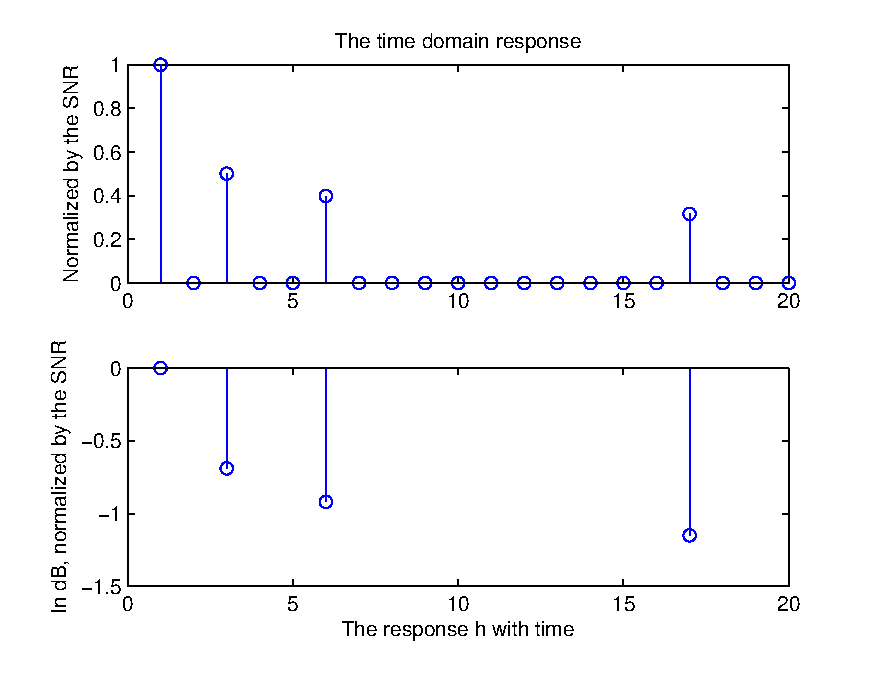
\includegraphics[width=0.8\linewidth]{1.eps}
		\caption{原始波形图}
\end{center}
\end{figure}
\begin{figure}[!h]
\begin{center}
		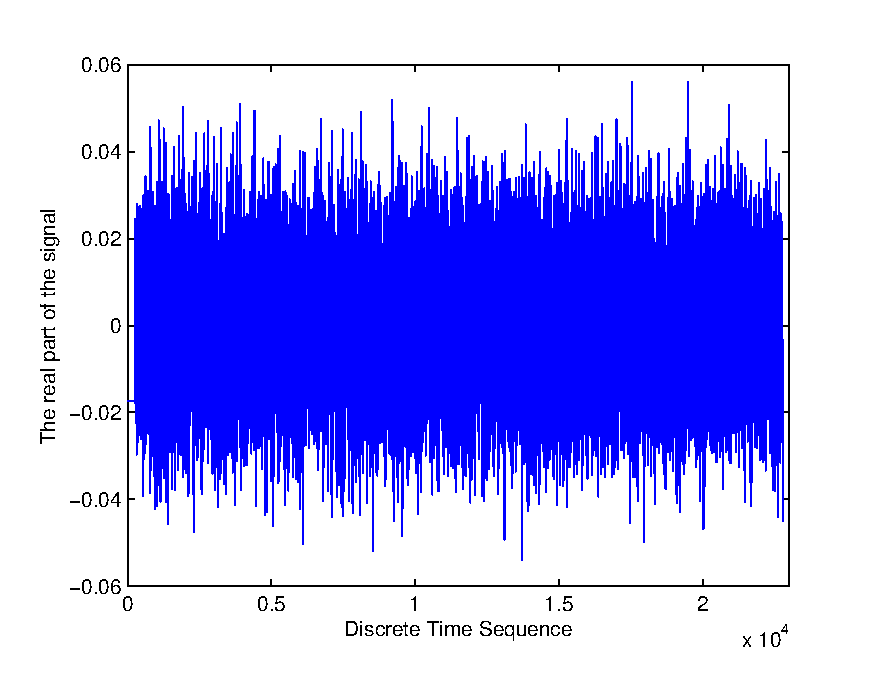
\includegraphics[width=0.8\linewidth]{2.eps}
		\caption{采样波形,采样频谱}
\end{center}
\end{figure}
\begin{figure}[!h]
\begin{center}
		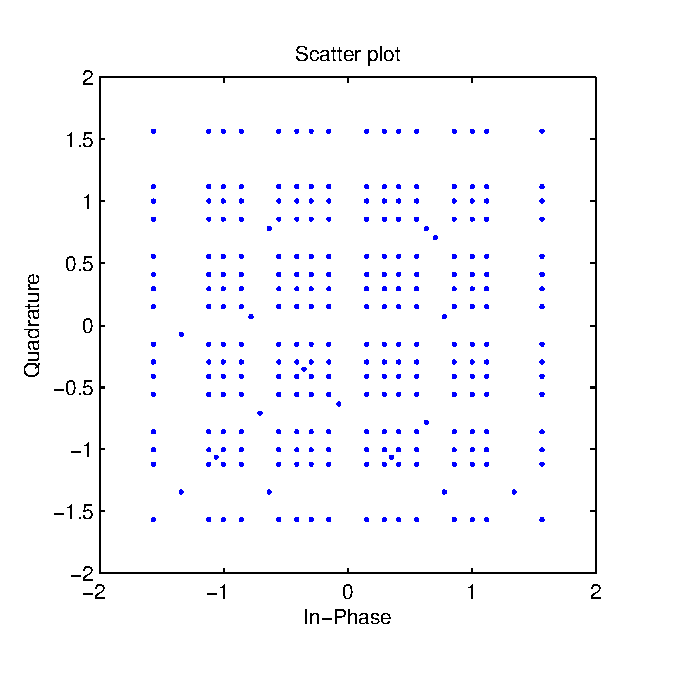
\includegraphics[width=0.8\linewidth]{3.eps}
		\caption{重构波形,重构频谱}
\end{center}
\end{figure}
\begin{figure}[!h]
\begin{center}
		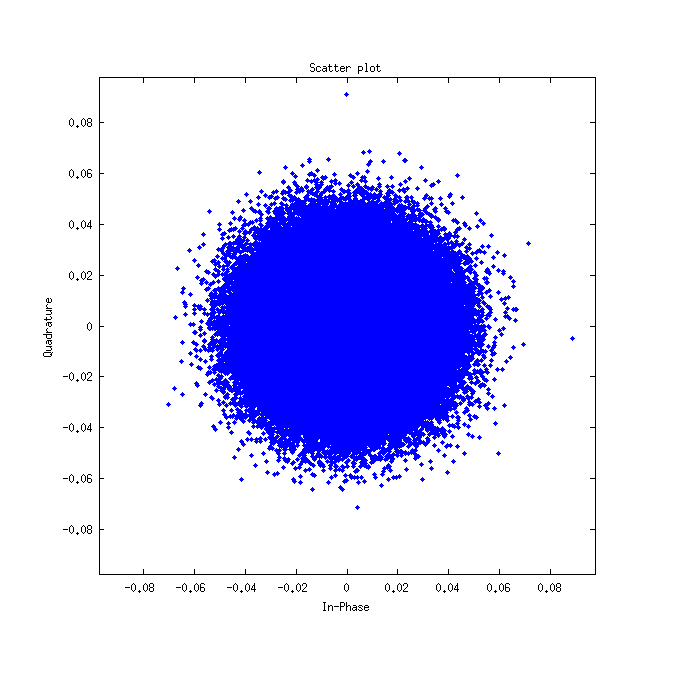
\includegraphics[width=0.8\linewidth]{4.eps}
		\caption{采样量化重构后的波形及频谱}
\end{center}
\end{figure}
\begin{figure}[!h]
\begin{center}
		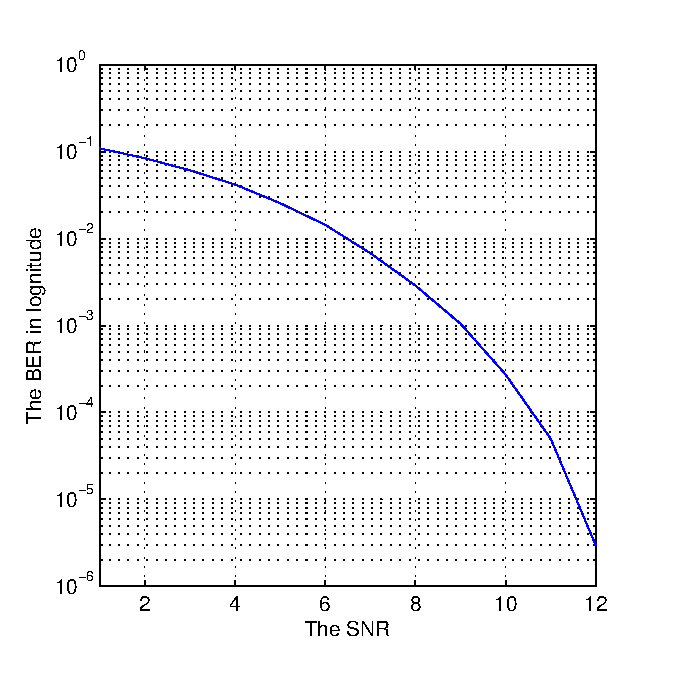
\includegraphics[width=0.8\linewidth]{5.eps}
		\caption{使用n=5重构误差波形及频谱}
\end{center}
\end{figure}
\begin{figure}[!h]
\begin{center}
		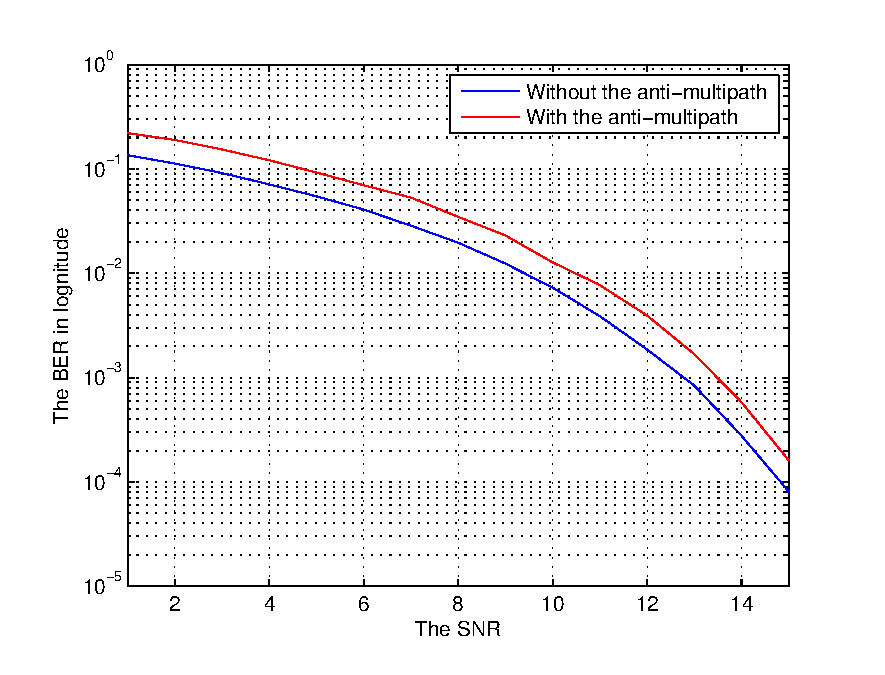
\includegraphics[width=0.8\linewidth]{6.eps}
		\caption{使用n=15重构误差波形及频谱}
\end{center}
\end{figure}
